%%%%%%%%%%%%%%%%%%%%%%%%%%% asme2ej.tex %%%%%%%%%%%%%%%%%%%%%%%%%%%%%%%
% Template for producing ASME-format journal articles using LaTeX    %
% Written by   Harry H. Cheng, Professor and Director                %
%              Integration Engineering Laboratory                    %
%              Department of Mechanical and Aeronautical Engineering %
%              University of California                              %
%              Davis, CA 95616                                       %
%              Tel: (530) 752-5020 (office)                          %
%                   (530) 752-1028 (lab)                             %
%              Fax: (530) 752-4158                                   %
%              Email: hhcheng@ucdavis.edu                            %
%              WWW:   http://iel.ucdavis.edu/people/cheng.html       %
%              May 7, 1994                                           %
% Modified: February 16, 2001 by Harry H. Cheng                      %
% Modified: January  01, 2003 by Geoffrey R. Shiflett                %
% Use at your own risk, send complaints to /dev/null                 %
%%%%%%%%%%%%%%%%%%%%%%%%%%%%%%%%%%%%%%%%%%%%%%%%%%%%%%%%%%%%%%%%%%%%%%

%%% use twocolumn and 10pt options with the asme2ej format
\documentclass[twocolumn,11pt]{asme2ej}
%% for loading postscript figures
\usepackage[T1]{fontenc}
\usepackage{graphics}
\usepackage{graphicx}
\usepackage{amsmath}
\usepackage{array}
\usepackage{multirow}
\usepackage{color}
\usepackage{numprint}
%% The class has several options
%  onecolumn/twocolumn - format for one or two columns per page
%  10pt/11pt/12pt - use 10, 11, or 12 point font
%  oneside/twoside - format for oneside/twosided printing
%  final/draft - format for final/draft copy
%  cleanfoot - take out copyright info in footer leave page number
%  cleanhead - take out the conference banner on the title page
%  titlepage/notitlepage - put in titlepage or leave out titlepage
%  
%% The default is oneside, onecolumn, 10pt, final

\newcommand\MyBox[1]{%
  \fbox{\parbox[c][.7cm][c]{.7cm}{\centering #1}}%
}
\newcommand\MyVBox[1]{%
  \parbox[c][.7cm][c]{1cm}{\centering\bfseries #1}%
}
\newcommand\MyHBox[2][\dimexpr.7cm+2\fboxsep\relax]{%
  \parbox[c][1cm][c]{#1}{\centering\bfseries #2}%
}
\usepackage{etoolbox}
\newcommand\MyTBox[3]{%
  \MyVBox{#1}
  \renewcommand*\do[1]{\MyBox{##1}\hspace*{-\fboxrule}}
  \docsvlist{#2}
  \MyBox{#3}\par\vspace{-\fboxrule}
}

\title{Using Neural Network to Intrusion Detection System}

%%% first author
\author{Cristian Lepore
    \affiliation{
	Course of Intelligent Systems\\
	M.S. in Computer Science\\
	Department of Computer Science\\
	University of Milan\\
    Email: cristian.lepore@studenti.unimi.it\\
    Mobile: +39 340 8071774
    }	
}


\begin{document}

\maketitle    

%%%%%%%%%%%%%%%%%%%%%%%%%%%%%%%%%%%%%%%%%%%%%%%%%%%%%%%%%%%%%%%%%%%%%%
\begin{abstract}
{\it \centering \textbf{Abstract}\\
Intrusion Detection System (IDS) predominantly works for detecting malicious attacks to computer network. In this project, we propose some IDS models based on Artificial Neural Network and clustering techniques. ANNs can only be built if there is availability of an effective dataset. A dataset with a sizable amount of quality data which mimics the real world, can help to train and test an intrusion detection system. We will introduce the NSL-KDD dataset. It has been used to study the effectiveness of the neural network-based classification algorithm to detect anomalies in the network traffic patterns. The entire analysis has been conducted using Matlab.
}
\\\\{
\textit{Keywords -- Intrusion Detection System, Artificial Neural Network, NSL-KDD dataset.}
}
\end{abstract}

%%%%%%%%%%%%%%%%%%%%%%%%%%%%%%%%%%%%%%%%%%%%%%%%%%%%%%%%%%%%%%%%%%%%%%

\section{Introduction}

%In recent years, the explosion of the Internet and the advent of ubiquitous technologies have
%revolutionized the world of computing, leading to limitless opportunities and possibilities. However, this effort also comes with the risk of malicious intrusions into the system that can jeopardize the system's data and resources.
Firewalls represent the most widely used security mechanisms in corporate networks but they can only protect from outside intruders. Hence, it is very important to have additional protection mechanisms in the internal host and network to prevent unauthorized access and possible inside threats. A key activity is called \textit{Intrusion Detection} and consists of monitoring a system or a network. Intrusion Detection Systems -- breafly IDSs -- fulfill such a purpose by breaking intrusive behaviors and consequently informing the security specialists.

In practical way, it is not possible to provide a complete prevention. However, it is viable to detect these intrusion attempts so that some actions may be taken to repair the damage.
%The field of information security has grown and evolved significantly in recent years in order to prevent and control information security threats. A plethora of exploits plagues computer networks ranging from zero-day exploits to computer worms and viruses capable of inflicting mass level infections and damages. In order to prevent these threats it is necessary to analyze the network packets and data to determine the attack methods used and the identity of who realized the attack. With the aim to reduce the problem, several developed solutions have been proposed, such as the use of robust cryptography, authentication systems, antivirus, firewalls, in addition to the \textit{Intrusion Detection Systems} (known as IDS systems). 
IDS goal is to identify unauthorized activity by inspecting individual machines and/or inbound network traffic. They are also important in order to understand new attacks and how they work so that an immediate response can be taken to prevent similar attacks. Snort\footnote{Snort is an open source project created by Martin Roesch. The project is maintained by Sourcefire and they created an easy to use command line tool to implement rulesets.} is an example of a well-known IDS product available for several platforms including Windows, Linux and MAC.

Despite, there are two types of IDSs: Network Based and Host Based, in this project we'll address only the Network Based IDS.
%\begin{list}{$\circ$}{}
%	\item Network Based IDS; using to detect network attacks by analyzing the payload.
%	\item Host Based IDS; using to detect local attacks before they hit the network.
%\end{list}
%
%In this project we will introduce the term IDS to refer only to Network Based IDS.

\subsection{Objective}

Our objective is to build an IDS model in order to separate safe connections from threats. We used IDS systems with \textit{Artificial Neural Networks} -- ANNs -- in order to classify possible malicious activities with high accuracy and once incorrectly classifying some data, they learnt from their own mistakes and improve their efficiency. We also made comparison with a clustering algorithm to see how well they perform with zero-day attacks.

The rest of this project is organized as follows: Section II presents the state-of-the-art. Section III reports the employed classification techniques. Section IV shows the  key activities to create the model. Final results and tests are depicted in section V, with conclusions reported in section VI.

%%%%%%%%%%%%%%%%%%%%%%%%%%%%%%%%%%%%%%%%%%%%%%%%%%%%%%%%%%%%%%%%%%%%%%

\section{State-of-the-art}

%A typical IDS architecture consists of four main components, namely, Sniffer, Preprocessor, Detection Engine, and Alerts Logger (as shown in Figure 1).
%\begin{figure}[h]
%\centering
%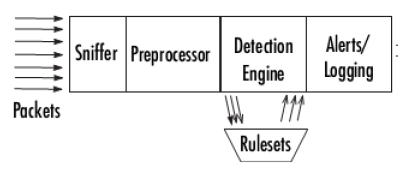
\includegraphics[scale=0.77]{IDS_architecture.png}
%\caption{IDS architecture}
%\end{figure}
%The sniffer is responsible for capturing the network traffic and passes the captured packets to the preprocessor. The preprocessor is responsible for sorting through the received packets and determining their types, i.e. tcp, udp or icmp. Once the packet is determined to have a particular type it is then sent to the detection engine. The detection engine matches the packet header and content against a set of rules. If the packet matches one or more rules in the detection engine, an alert will be triggered and stored in a log file or a database.

Network-based IDS systems detect attacks by capturing and analyzing network packets, from
sensors placed at various points in a network. In general, there are two primary models to analyzing events to detect attacks: \textit{misuse detection} and \textit{anomaly detection}. In misuse detection model IDS detect intrusions by looking for activity that corresponds to known signatures of intrusions or vulnerabilities. Anomaly detection instead, detects intrusions by searching abnormal network traffic and they have the ability to detect symptoms of attacks without specifying model of attacks. We want to work on this second class of detection (anomaly detection).

The majority of tools available today refer to the misuse detection model, meaning that administrators need to regularly update vulnerabilities database. Instead, commercial tools available for anomaly detection have limitations in detecting real intrusions, and Neural Network is a efficient way to improve the performances of these IDS systems. Applying the Neural Network approach to Intrusion Detection, we first have to expose NN to normal data and to attacks to automatically adjust coefficients of the NN during the training phase. Performance tests are then conducted with real network traffic and attacks.

%To do so, we should consider an Intrusion Detection System as a pattern recognition system. Intrusion scenarios are encoded into patterns, and incoming events are verified by matching them against these patterns.

%%%%%%%%%%%%%%%%%%%%%%%%%%%%%%%%%%%%%%%%%%%%%%%%%%%%%%%%%%%%%%%%%%%%%%

\section{Employed classification techniques}

In this section we briefly review the data mining
techniques that are employed in our models to evaluate performances and make comparisons.
%Artificial Neural Network (ANN) is an information processing system that mimics the human brains. It consists of a large number of interconnected processing nodes (called neurons) collaborating with each other to solve a specific task.
%Each node has a specific activation function. The output of each node in a given layer is fed as an input to all other nodes in the adjacent layer. The neural network learning process can therefore be considered as an optimization task.
\\\\
\textit{Feedforward Neural Network} -- They consist of a series of layers. The first layer has a connection from the network input. Each subsequent layer has a connection from the previous layer. The final layer produces the network's output. A feedforward network with enough neurons in the hidden layers, can fit any finite input-output mapping problem. 
\\\\
\textit{Radial basis function} -- Similarly to the previous one, they consist of two layers. A hidden radial basis layer and an output linear layer. The transfer function is described by a radial basis function with its maximum to 1 when the input is 0. %Figure 2 depicts the overall architecture of the %proposed ANN model.
%\begin{figure}
%\centering
%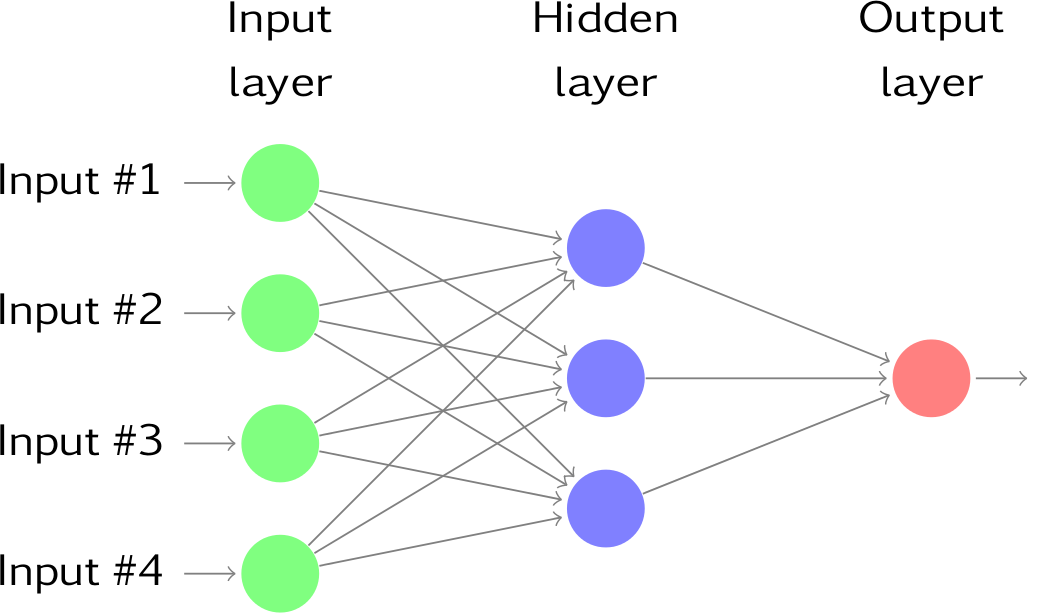
\includegraphics[scale=0.22]{ANN_model.png}
%\caption{Feed-forward NN architecture}
%\end{figure}
%In brief the neural network model consists of the following basic steps: 
%\begin{itemize}
%	\item 1. Feed the neural network with inputs
%	\item 2. Comparison of the output
%	\item 3. Alter the weights of the neurons
%\end{itemize}
%
%In this project, we present results using the feed-forward neural network and the RBF to develop an IDS model. Fig. 1 depicts the overall architecture of the proposed ANN based 
%IDS model.
%\begin{figure}
%\centering
%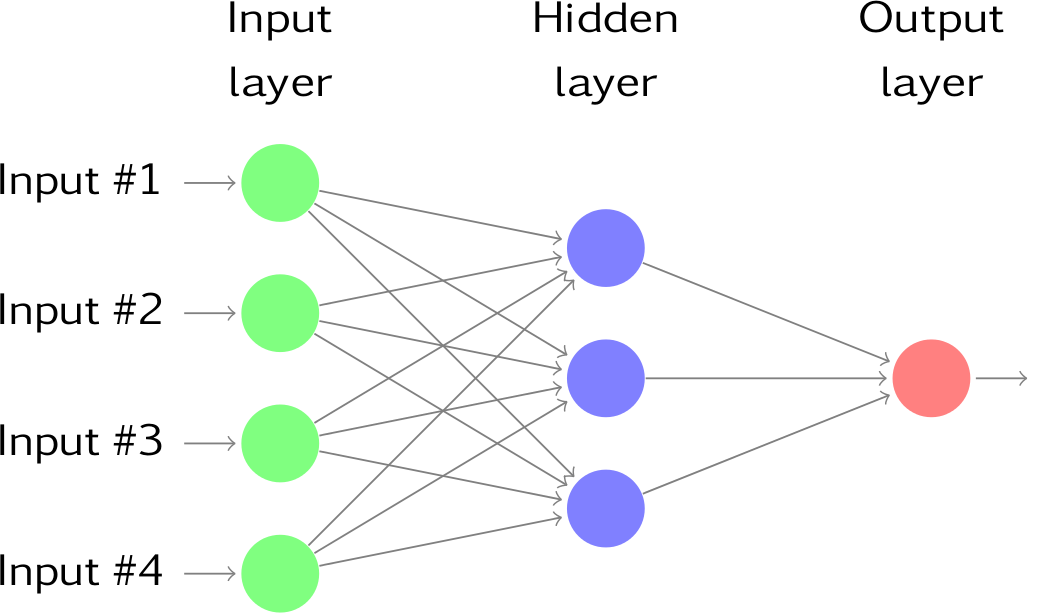
\includegraphics[scale=0.24]{ANN_model.png}
%\caption{Artificial Neural Network Model}
%\end{figure}
%The model consists of an input layer, a single hidden layer and an output layer. The number of nodes in the input and the hidden layers are set to number of feature in the input feature vector. Similarly, the number of nodes in the output layer is set to the number of desired output classes. The model may contains several plies in the hidden layer but each node in a given layer is connected to another node of a different layer. Each connection has an associated weight value given by the link between two adjacent nodes. Using the back-propagation we can obtain the right configuration of the parameter for our ANN.
\\\\
\textit{Clustering Technique} -- Clustering data is an excellent application for neural networks. This process involves grouping data by similarity. \textit{Self-organizing maps} algorithm is a unique method in that it combines the goals of the projection and clustering algorithms. It can be used at the same time to visualize the clusters in a dataset,  and to present the set on a two dimensional map.

%For this purpose we chose the \textit{K-means clustering} because is one of the simplest unsupervised learning algorithms able to give good performances. The procedure tries to classify a given data set through a certain number of clusters (assume K clusters) fixed apriori. The main idea is to define K centers, one for each cluster. The better choice is to place them as much as possible far away from each other. As final result we obtain a partitioning of the data space into Voronoi cells.
%The unlabeled data from the large dataset can be classified in an unsupervised manner using clustering algorithms. K-means is one of the simplest unsupervised learning algorithms that solve the well-known clustering problem. It is an unsupervised data mining technique for intrusion detection easy to implement. The procedure follows a simple and easy way to classify a given data set through a certain number of clusters (assume k clusters) fixed apriori. The main idea is to define k centers, one for each cluster. The better choice is to place them as much as possible far away from each other.  
%
%
%
%The next step is to take each point belonging to a given data set and associate it to the nearest center. When no point is pending, the first step is completed and an early group age is done. At this point we need to re-calculate k new centroids as barycenter of the clusters resulting from the previous step. After we have these k new centroids, a new binding has to be done between the same data set points and the nearest new center. A loop has been generated. As a result of this loop we may notice that the k centers change their location step by step until no more changes are done or in other words centers do not move anymore.

%%%%%%%%%%%%%%%%%%%%%%%%%%%%%%%%%%%%%%%%%%%%%%%%%%%%%%%%%%%%%%%%%%%%%%

\section{Methodology}

Let us focus on the implementation of the model. The IDS system proposed in this work is the result of several key activities depicted in figure 1.
\begin{figure}[h]
\centering
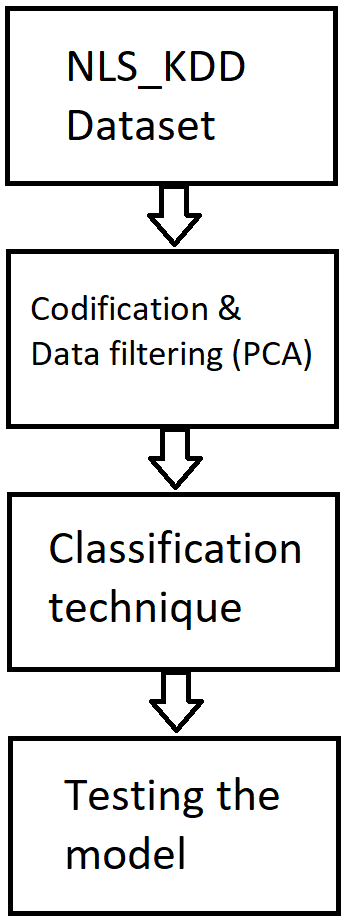
\includegraphics[scale=0.25]{Methodology2.png}
\caption{Key activities}
\end{figure}
\\\\
\textit{1. Dataset} -- The dataset used for training the model is known as NSL-KDD, which is provided by DARPA\footnote{DARPA stands for Defense Advanced Research Projects Agency. It is part of the US Department of Defense responsible for the development of emerging technologies for use by the military.}. It is a refined version of its predecessor and it has been widely used for simulating and testing the IDS systems. A second database containing new attack patterns has been used for testing. For more details about the datasets, please refer to the section 5.1 under Experiments and Results. Each record is described by 42 attributes unfolding different features of the flow and a label assigned to each either as an attack type or as normal.\\\\
\textit{2. Pre-prosessing} -- To facilitate the analisys, the whole dataset has been splitted by two. In one side the input matrix with the 41 attributes that characterize the connection; on the other hand the target matrix which contains only the labels.\\\\
\textit{3. Codification} -- Neural network works best only on numerical data, which requires conversion of the textual data in the dataset to a numerical value. For this reason the variables 'protocol type', 'service', 'flag' and 'label' (from the input and target matrix) need to be converted into numerical values. To do the required conversion, a slight Matlab program has been developed in order to map the text into numbers. The next table shows how we mapped variables into numerical attributes. The attack classes are mapped with a 5 digits and constitutes the output value. The other attributes are simply mapped with numerical values in a range from 1 to 81.
\\\\
\begin{tabular}{cc|c|c|c|c|l}
%Header
\cline{1-3}
\multicolumn{1}{ |c  }{\multirow{1}{*}{\textbf{Type of attribute}} } &
\multicolumn{1}{ |c| }{\textbf{Attribute}} & \textbf{Mapping}
\\ \cline{1-3}

\cline{1-3}
\multicolumn{1}{ |c  }{\multirow{5}{*}{Label}} &
\multicolumn{1}{ |c| }{Normal} & 10000

\\ \cline{2-3}
\multicolumn{1}{ |c| }{} & DoS & 01000

\\ \cline{2-3}
\multicolumn{1}{ |c| }{} & Probe & 00100

\\ \cline{2-3}
\multicolumn{1}{ |c| }{} & R2L & 00010

\\ \cline{2-3}
\multicolumn{1}{ |c| }{} & U2R & 00001
\\ \cline{1-3}

%Seconda fila
\multicolumn{1}{ |c  }{\multirow{3}{*}{Protocol type} } &
\multicolumn{1}{ |c| }{TCP} & 1

\\ \cline{2-3}
\multicolumn{1}{ |c| }{} & UDP & 2

\\ \cline{2-3}
\multicolumn{1}{ |c| }{} & ICMP & 3
\\ \cline{1-3}

%Terza fila
\multicolumn{1}{ |c  }{\multirow{1}{*}{Flag} } &
\multicolumn{1}{ |c| }{All flags} & 5 to 15
\\ \cline{1-3}

%Quarta fila
\multicolumn{1}{ |c  }{\multirow{1}{*}{Service} } &
\multicolumn{1}{ |c| }{All services} & 16 to 81
\\ \cline{1-3}
\end{tabular}
\\\\\\
The whole mapping process took almost 45 minutes.\\\\
\textit{4. Normalization} -- In ANN we need to normalize the inputs, otherwise the network will be ill-conditioned. It is done to have the same range of values for each of the inputs to the ANN model. This can guarantee stable convergence of weight and biases.\\\\
\textit{5. Features selection} -- High dimensional data are very common in network sniffing due to the multiple features that the sniffer is able to capture. These attributes are not always convenient and one approach is to reduce the dimension of the feature space using a well-suited technique namely Principal Component Analysis (PCA). Its outcome is to project a feature space onto a smaller subspace. %The main idea is to separates link traffic measurements into sub regions representing normal and abnormal traffic.%
By selecting the most important features -- called principal components -- we improved performances and saved computational time. That was a very important goal to reach. Thus, the final dataset undergo a dimensionality reduction and contains 15 features.\\\\
\textit{6. Classification techniques} -- For the analysis, Matlab 2018a v9.4.0 has been used with the integrated Neural Network toolbox for pattern recognition. The system is a CPU Intel Core i5 @1.7GHz and 8GB of RAM. The operating system is a Microsoft Windows 10 Enterprise edition.%In K-fold cross validation, the data set is divided into k subsets. In every iteration, one of the k subsets is considered as the test set and the other k $-$ l subsets are considered as training set. The advantage of this method is that the data point will be in the test set at least once and in the training set k $-$ l times.

The tests have been conducted employing a feedforward neural network (shown in figure 2), a RBF network and a clustering technique as explained in section 5.2 under Training and Testing. 
\begin{figure}[h]
\centering
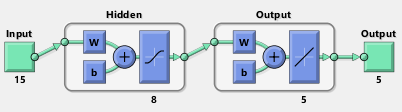
\includegraphics[scale=0.8]{ANN_model2.png}
\caption{Feedforward NN model}
\end{figure}
K-fold Cross-validation has been adopted. It is a well-known technique that uses only a partial dataset for training while the other records are used to measure the performance of the model. \\\\
\textit{7. Intrusion detection evaluation} -- In this project, we consider the \textit{Detection rate} (DR) as principal metric. This parameter is mostly adopted in literature.
$$ Detection\ rate\ (DR)= \frac{TN}{TN + FP} $$ To compare results, we also used the \textit{Accuracy} rate and \textit{Precision} rate.

%%%%%%%%%%%%%%%%%%%%%%%%%%%%%%%%%%%%%%%%%%%%%%%%%%%%%%%%%%%%%%%%%%%%%%

\section{Experiments \& Results}

Let's talk more in detail about the dataset and the results that we obtained from the trained IDS models. Some experiments are proposed with the aim to provide the optimal solution for the classification problem.

\subsection{Dataset}

NSL-KDD is a public dataset created in 2007 by sniffing packets during a day-by-day network activity. The simulation network was made of a factitious military network consisting of three target machines running various operating systems and services. Additional three machines were then used to spoof different IP addresses to generate traffic. Finally, a sniffer recorded all network traffic using the TCP dump format. The total simulated period was seven weeks.

It can be considered as a perfect representative of an existing real world scenario \footnote{There is a lack of this kind of databases because people are concerned about their privacy when sniffing private communications.}. Furthermore, the number of records is reasonable and makes it affordable to run the experiments on the complete set without the need to randomly select a small portion. Each record represents a connection intercepted through the network. 41 attributes to describe it (i.e. protocol type, number of bytes, header, etc..) and a label assigned to each either as a specific type of attack or as normal.

Each pattern of the NSL-KDD dataset falls into any one of the following classes, namely, Normal and four different kinds of attacks such as Probe, Denial of Service (DoS), Remote to Local (R2L) and User to Root (U2R):
\begin{itemize}
\item \textit{A. DoS Attack}

attacks which attempt to crash the victim host by exhausting its computing or memory resources, so it cannot handle legitimate requests.\\

\item \textit{B. Probe Attack}

attacks scanning computer networks to gather information or find known vulnerabilities, which are exploited for further or future attacks.\\

\item \textit{C. R2L Attack}

attacks in which an unauthorized user can gain local access through bypassing normal authentication and executing commands on the victim machine.\\

\item \textit{D. U2R Attack}

attacks in which a normal user with login access can gain the privileges of root users by bypassing normal authentications.\\

\end{itemize}

\subsubsection{Distribution of class label}

Two databases have been employed has part of the NSL-KDD packet. One for training and testing the model on known attacks using the k-folds cross validation and a second one employed solely to test the model's behavior on unknown attacks. NSL-KDD Train contains 24 different attack patterns plus the normal connections; in contrast the NSL-KDD Test consists of 37 different attack patterns and the normal connections. It means that using the second database for testing the model, it tries to categorize attacks that has never seen before. In a nutshell, these records simulate a "zero-day attack". The total amount of these zero-day attacks enclosed in the Test database is \numprint{3752} and it constitute the 30\% of the database patterns. All the patterns for both databases fall into 5 main classes as reported before. Table 1 and figure 3 represent the distribution of the class labels for both databases.
\begin{table}[t]
\caption{Distribution of class label}
\begin{center}
\label{table_ASME}
\smallskip\noindent
\resizebox{\linewidth}{!}{%
\begin{tabular}{l l l} % put some space after the caption
\hline
\textbf{Type of connection} \hspace{1cm}& \textbf{NSL-KDD Train} \hspace{1cm}& \textbf{NSL-KDD Test}\\
\hline
Normal & \numprint{67343} & \numprint{9711}\\
DoS & \numprint{45927} & \numprint{7460}\\
Probe & \numprint{11656} & \numprint{2421}\\
R2L & \numprint{995} & \numprint{2885}\\
U2R & \numprint{52} & \numprint{67}\\
\hline
\textbf{Total} & \textbf{\numprint{125973}} & \textbf{\numprint{22544}}\\
\hline
\end{tabular}}
\end{center}
\end{table}
\begin{figure}[h]
\centering
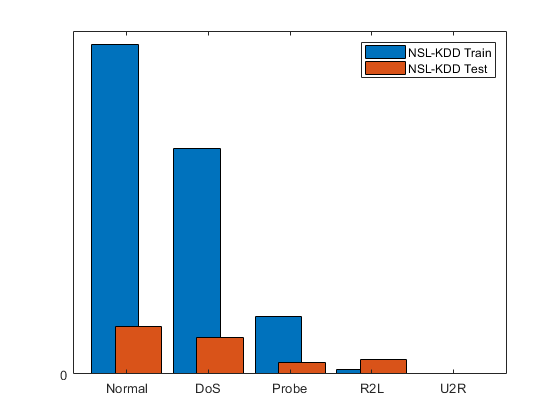
\includegraphics[scale=0.52]{class_label2.png}
\caption{Distribution of class label}
\end{figure}
They contain some low frequency attack classes like R2L and U2R. As a result the neural network may not use these instances during the training process. This is exactly what we expect to have in a real scenario because some types of threats like DoS and DDoS are more likely to happen than others.

%%%%%%%%%%%%%%%%%%%%%%%%%%%%%%%%%%%%%%%%%%%%%%%%%%%%%%%%%%%%%%%%%%%%%%

\subsection{Training and Testing}

The train dataset was splitted into 10 non duplicated subsets and any nine of the subsets will be used for training the model and the remaining one for testing. This is termed as \textit{10-fold cross validation} as explained before.

\subsubsection{PCA Analysis}

Before apply any neural network models, PCA analysis was first employed to the original data to explore possibilities for data reduction in further predictions. We want to demonstrate that a combination between PCA and the ANN performs well even if a few axes are considered to represent the records. 

PCA analysis was executed according to the various situations. Figure 4 shows the variance estimation of the first ten principal components. 
\begin{figure}[h]
\centering
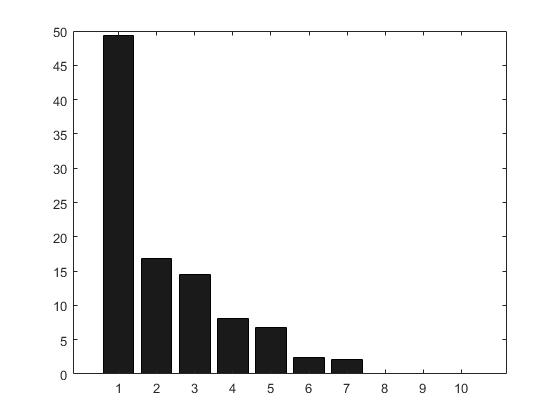
\includegraphics[scale=0.52]{Variance_estimation.png}
\caption{Variance estimation of the principal
components}
\end{figure}
As expected, the graph describes an elbow curve. The five principal components having a cumulative variation of more than 90\% are retrained and the others 36 (the remaining 10\% of the cumulative variation) were tested to seek the optimal number of axes.

Using the classification techniques, we experimented the dataset on a new feature space generated by several PCA's axes. We have performed the different experiments considering 5, 8, 10, ..., 41 axes, because the cumulative variation with 5 axes is already more than 90\%. Figure 5 reports the accuracy rate varying the number of the principal components of the feedforward, RBF and SOM network.
\begin{figure}[h]
\centering
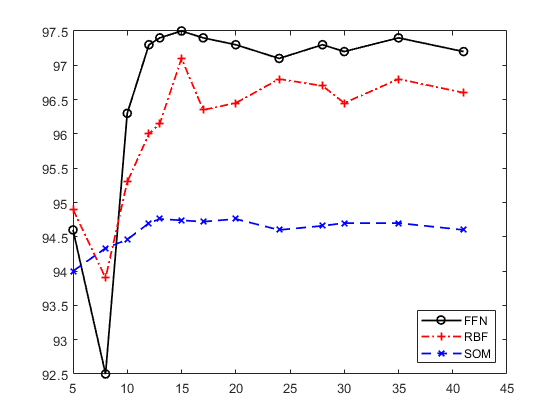
\includegraphics[scale=0.52]{PCA_RBF.png}
\caption{Accuracy rate by changing the number of axes}
\end{figure}
For every neural network there is not much difference in the accuracy rate considering more than thirteen axes; that is where the graph become flat. The result shows that 15 axes are slightly better than any other. In general using fifteen axes, we obtain a higher accuracy that we would have using the entire database. In addition, the computation time is reduced by a factor of approximately three (from 41 to 15) when considering 15 principal components. Hence, it is better to reduce the space on which the connection records are represented before applying any learners. So in the subsequent tests, we always consider a database with only 15 features.

%%%%%%%%%%%%%%%%%%%%%%%%%%%%%%%%%%%%%%%%%%%%%%%%%%%%%%%%%%%%%%%%%%%%%%

\subsubsection{Feedforward with PCA}

To evaluate the performance of the employed feedforward network, experiments varying the number of neurons in the hidden ply were conducted. Increasing the number of neurons, increases as well the demand for computational capacity and the overfitting occurrence. Table 2 shows the obtained results training the network for 100 epochs. We have the best performance using 8 neurons. Buy the way, the R2L detection rate is always under the 10\% for every model. Furthermore, increasing the number of neurons we observe some overfitting occurrences. 

We report the confusion matrix for the proposed model with 8 neurons.
\begin{table}[t]
\renewcommand{\arraystretch}{1.7}
\caption{Results for simulation of ANN}
\begin{center}
\smallskip\noindent
\resizebox{\linewidth}{!}{%
\label{table_ASME}
\begin{tabular}{l c c c c c c} % put some space after the caption
\hline
\textbf{Detection rate} \hspace{0cm}& \textbf{FFN-2N} \hspace{0cm}& \textbf{FFN-8N} \hspace{0cm}& \textbf{FFN-12N} \hspace{0cm}& \textbf{FFN-20N}\\
\hline
Hidden layer & 2 & \textbf{8} & 12 & 20\\
Time & 5'30'' & \textbf{6'20''} & 15'10'' & 30'30''\\
Normal & 85.0\% & \textbf{99.1\%} & 99.0\% & 98.9\%\\
DoS & 88.1\% & \textbf{98.3\%} & 97.4\% & 97.3\%\\
Probe & 78.8\% & \textbf{93.2\%} & 93.7\% & 94.3\%\\
R2L & 0.0\% & \textbf{7.7\%} & 6.2\% & 7.4\%\\
U2R & 0.0\% & \textbf{0\%} & 0\% & 0\%\\
\hline
\textbf{Accuracy} & 84.85\% & \textbf{97.51\%} & 97.22\% & 97.10\%\\
\textbf{DR} & 83.56\% & \textbf{98.98\%} & 98.85\% & 98.73\%\\
\hline
\end{tabular}}
\end{center}
\end{table}

\smallskip\noindent
\resizebox{\linewidth}{!}\\
\cline{2-7}
\multirow{2}{*}{}& Normal & \textbf{\numprint{66768}} & \numprint{756} & \numprint{640} & \numprint{904} & \numprint{51} & 96.6\\
\cline{2-7}
& DoS & \numprint{221} & \textbf{\numprint{45125}} & \numprint{135} & \numprint{11} & \numprint{0} & 99.2\\
\cline{2-7}
& Probe & \numprint{333} & \numprint{46} & \textbf{\numprint{10866}} & \numprint{3} & \numprint{1} & 96.6\\
\cline{2-7}
& R2L & \numprint{21} & \numprint{0} & \numprint{15} & \textbf{\numprint{77}} & \numprint{1} & 68.1\\
\cline{2-7}
& U2R & \numprint{0} & \numprint{0} & \numprint{0} & \numprint{0} & \textbf{\numprint{0}} & \numprint{0}\\
\cline{2-7}
\multicolumn{1}{c}{} & \multicolumn{1}{c}{Total \%} & \multicolumn{1}{c}{99.1} & \multicolumn{1}{c}{98.3} & \multicolumn{1}{c}{93.2} & \multicolumn{1}{c}{7.7} & \multicolumn{1}{c}{0} & \multicolumn{1}{c}{\textbf{97.5}} \\\end{tabular}}
\\\\

The cell values report the number of pattern occurrences. The minimum accuracy of the classification has been observed for class 5 (U2R), which is 0\%. This is probably due to the reduced amount of samples currently in the database for this pattern. See table 3 for more statistics.

The false positive rate -- 0.46\% -- (number of normal connections that are incorrectly classified as intrusion attacks) is lower than false negative -- 1.86\% -- (number of intrusion attacks that are incorrectly classified as normal connection). In general, a false negative is the most dangerous state since the security professional has no idea that an attack took place.

%%%%%%%%%%%%%%%%%%%%%%%%%%%%%%%%%%%%%%%%%%%%%%%%%%%%%%%%%%%%%%%%%%%%%%

\subsubsection{RBF with PCA}

We design a two-layer network, setting the goal for the MSE to 0.01 and the radial function's spread to 10. We didn't notice any significant performance improvement by changing the function's spread. The larger spread is, the smoother the function approximation. Too large a spread means a lot of neurons are required to fit a fast-changing function. Too small a spread means many neurons are required to fit a smooth function, and the network might not generalize well. During the training process the network increases the number of neurons by 50 each round until the mean squared error falls below the goal.

This analysis is greedy of memory, so we have randomly selected the 10\% of the records producing a smaller database of \numprint{12597} patterns. From the confusion matrix, we see a false positive rate -- 2.14\% -- greater than the false negative -- 0.58\%.

\smallskip\noindent
\resizebox{\linewidth}{!}\\
\cline{2-7}
\multirow{2}{*}{}& Normal & \textbf{\numprint{6674}} & \numprint{23} & \numprint{43} & \numprint{6} & \numprint{0} & 98.9\\
\cline{2-7}
& DoS & \numprint{135} & \textbf{\numprint{4483}} & \numprint{8} & \numprint{0} & \numprint{0} & 96.9\\
\cline{2-7}
& Probe & \numprint{54} & \numprint{31} & \textbf{\numprint{1033}} & \numprint{1} & \numprint{0} & 92.3\\
\cline{2-7}
& R2L & \numprint{72} & \numprint{0} & \numprint{0} & \textbf{\numprint{26}} & \numprint{0} & 26.5\\
\cline{2-7}
& U2R & \numprint{8} & \numprint{0} & \numprint{0} & \numprint{0} & \textbf{\numprint{0}} & 0\\
\cline{2-7}
\multicolumn{1}{c}{} & \multicolumn{1}{c}{Total \%} & \multicolumn{1}{c}{96.1} & \multicolumn{1}{c}{98.8} & \multicolumn{1}{c}{95.3} & \multicolumn{1}{c}{78.8} & \multicolumn{1}{c}{0} & \multicolumn{1}{c}{\textbf{96.9}} \\\end{tabular}}
\\\\

In general, the main concern for IT System Administrators is related with the false negative rate. In contrast, false positive are an inconvenience at best and can cause significant issues. However, with the right amount of overhead, false positives can be successfully adjudicated; false negatives cannot. Compare with the previous model, the majority of R2L patterns are detected. See table 3 for more details.

\subsubsection{Self-organizing maps with PCA}

We employed a $20$x$20$ Kohonen's Self Organizing Map with an hexagonal topology to build a two dimensional map of patterns. We trained the network for 50 ephocs.
\\\\
\textit{Assigning Labels} -- In order to assign labels to SOM neurons we maintain a hit score matrix $h(i,j)$ where $i$ is the class label index and $j$ is the neuron index. As neuron $j$ gets selected as winning neuron for more input samples from class $i$, $h(i,j)$ score increases. After the SOM is trained, inputs from the training set are presented to determine the winning neurons. Hits score of the winning neuron for the given label (i.e. $h(i,j)$) is ranked assigning a higher score to a neuron that is closer to the input pattern in terms of Euclidean distance. Neurons are labeled with the class label, which has the highest hit score.
\\\\
\textit{Pattern visualization} -- To visualize the cluster structure, a graphic display called U-Matrix is used. It shows the distances between weight vectors of the neurons using a color scale. The colors in the regions containing the red lines indicate the distances between neurons. The darker colors represent larger distances, and the lighter colors represent smaller distances. 

Figure 6 shows the U-Matrix of the SOM with assigned labels. It is important to note that patterns can be assigned neurons on different regions of the SOM since different stages of a connection can exhibit different behavior. Analysis of the U-Matrix reveals that five regions emerge from the SOM shown. From left (Region 1), right (Region 2), lower (Region 3), center (Region 4) and upper left (Region 5).

\begin{figure}[h]
\centering
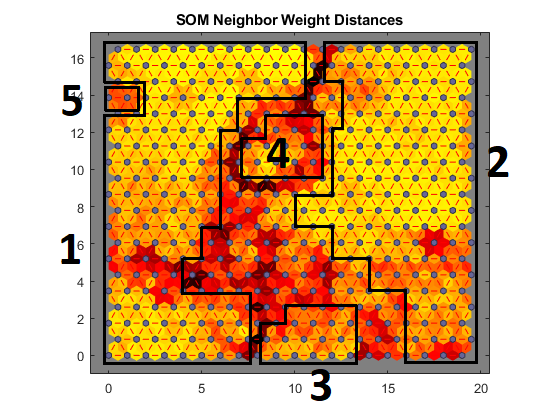
\includegraphics[scale=0.63]{U-Matrix2.png}
\caption{Pattern Map}
\end{figure}

Region 1, which is the larger Region, contains normal packets with the connections that are not classified as risky. On region 2, the denial of service attack where the attacker sends spoofed SYN packets. Region 3 and 4 are respectively Probe and R2L attacks. Finally the smaller area, that is very though to find, the User to Root attacks which have only 52 samples. Probe and denial of service attacks are commonly clustered together (namely Regions 2, 3). This is due to the fact that both type of attacks have observable impacts on network traffic.

On the other hand, Figure 7 shows the analysis of the above U-Matrix from the perspective of the 15 different features. They are visualizations of the weights that connect each input to each of the neurons. Darker colors represent larger weights. If the connection patterns of two inputs were very similar, the inputs are highly correlated.
\begin{figure}[h]
\centering
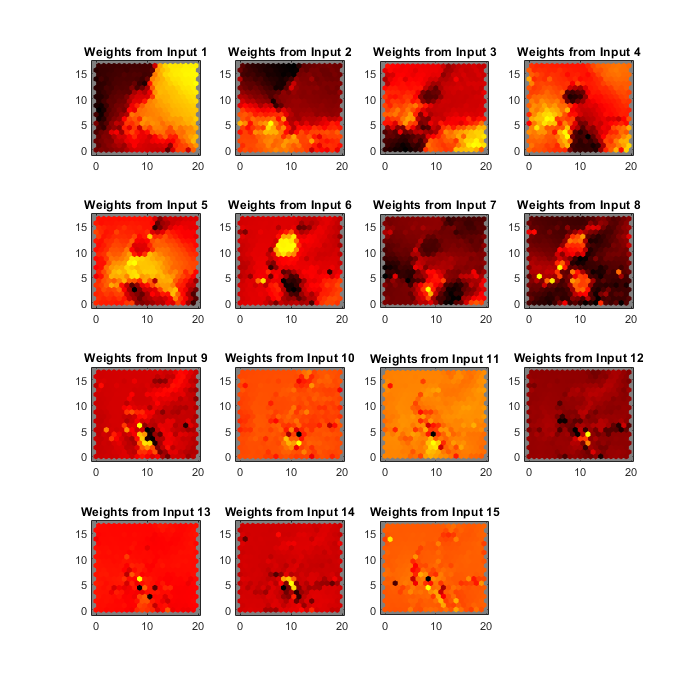
\includegraphics[scale=0.5]{U-Matrix_features.png}
\caption{Application of U-Matrix visualization to 15 features separately}
\end{figure}
\\\\
\textit{Accuracy} -- It implies the recognition of a pattern based on a given input to the SOM. Hence, it is calculated by presenting the input to the SOM and finding the winning neuron. If the winning neuron has the same label with the input, it is considered a correct identification otherwise it is a mistake. We report below the confusion matrix for the model. From the analysis, we noticed that the U2R attack type still remains undetected. By the way, the overall model's accuracy rate is $95.2\%$. Further metrics are available on table 3.

\smallskip\noindent
\resizebox{\linewidth}{!}\\
\cline{2-7}
\multirow{2}{*}{}& Normal & \textbf{\numprint{65299}} & \numprint{702} & \numprint{475} & \numprint{361} & \numprint{41} & 97.6\\
\cline{2-7}
& DoS & \numprint{782} & \textbf{\numprint{44549}} & \numprint{1758} & \numprint{0} & \numprint{0} & 94.6\\
\cline{2-7}
& Probe & \numprint{1018} & \numprint{659} & \textbf{\numprint{9414}} & \numprint{16} & \numprint{1} & 84.7\\
\cline{2-7}
& R2L & \numprint{244} & \numprint{17} & \numprint{9} & \textbf{\numprint{618}} & \numprint{10} & 68.8\\
\cline{2-7}
& U2R & \numprint{0} & \numprint{0} & \numprint{0} & \numprint{0} & \textbf{\numprint{0}} & 0\\
\cline{2-7}
\multicolumn{1}{c}{} & \multicolumn{1}{c}{Total \%} & \multicolumn{1}{c}{97.0} & \multicolumn{1}{c}{97.0} & \multicolumn{1}{c}{80.8} & \multicolumn{1}{c}{62.1} & \multicolumn{1}{c}{0} & \multicolumn{1}{c}{\textbf{95.2}} \\\end{tabular}}
\\\\

%%%%%%%%%%%%%%%%%%%%%%%%%%%%%%%%%%%%%%%%%%%%%%%%%%%%%%%%%%%%%%%%%%%%%%

\subsubsection{Analogies between models}

Let's step back for a moment to figure 5. It shown a comparison between the three different models changing the number of axes used for the test. The feedforward network (continuous line) gave the best performances. The other two networks never reached this level of accuracy but for both of them the shape of the curve is similar. In general considering the overall accuracy as the only metric, the RBF network behaves better than SOM but worse than feedforward network.

Let's take a look at the detection rate of the different input patterns shown on table 3. The best threats detection is reached with the RBF network (see the row namely "Attack" in the table); while feedforward got the best overall detection rate. Examining the false alarm rate (shown on figure 8) we see that a RBF model could be the best choice because of the low number of false negative alarms. In fact a false positive alarm can be mitigate using a double check (i.e. using a host-based IDS); in contrast, false negative cannot.

\begin{table}[t]
\caption{Metrics comparison}
\begin{center}
\label{table_ASME}
\begin{tabular}{l c c c} % put some space after the caption
\\\hline
\textbf{Detection rate \%} \hspace{0cm}& \textbf{FFN} \hspace{0cm}& \textbf{RBF} \hspace{0cm}& \textbf{SOM}\\
\hline
Time & 6'20'' & 90' & 83'\\
Normal & 99.1 & 96.1 & 97.0\\
DoS & 98.3 & 98.8 & 97.0\\
Probe & 93.2 & 95.3 & 80.8\\
R2L & 7.7 & 78.8 & 62.1\\
U2R & 0 & 0 & 0\\
\hline
\textbf{Accuracy} & 97.51 & 96.98 & 95.2\\
\textbf{DR} & 98.98 & 95.37 & 96.54\\
\textbf{Precision} & 95.99 & 98.73 & 97.31\\
\hline
\end{tabular}
\end{center}
\end{table}

\begin{figure}[h]
\centering
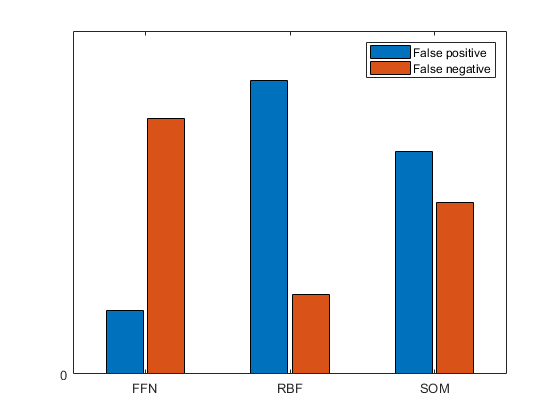
\includegraphics[scale=0.52]{Comparison_graph.png}
\caption{False alarm rate}
\end{figure}

\subsubsection{Zero-day attacks}

We want to test our employed models on a new class of patterns to see how well they perform with zero-day attacks. The test database contains known and unknown patterns as specified in section 5.1.1. In order to determine the best model as possible, we retrained our neural networks on the entire train database; so this time, cross validation hasn't been adopted.

The ability of our models to detect the right class for R2L and U2R attack types was very low, so we kept the analysis on a higher level, focusing on the system's ability to discriminate between normal connections (safe) and threats. If the IDS is able to split between safe and unsafe means that a security specialist has a clue that an attack is taking place also if he/she doesn't realize which kind of threat it is.

Table 4 reports a comparison between the three different classification techniques using only two labels (normal and attack) to evaluate the accuracy. Attack simply identify the bad connections, in contrast normal determine the good one. We see that the feedforward neural network performed better than any other but the overall accuracy is lower compared to the previous test. The false negative rate is quite high and probably is due to a bias toward the R2L class that has many samples.

\begin{table}[t]
\caption{Metrics comparison using NSL-KDD Test dataset}
\begin{center}
\label{table_ASME}
\begin{tabular}{l c c c} % put some space after the caption
\\\hline
\textbf{Detection rate \%} \hspace{0cm}& \textbf{FFN} \hspace{0cm}& \textbf{RBF} \hspace{0cm}& \textbf{SOM}\\
\hline
Normal & 93.0 & 88.7 & 96.7\\
Attack & 75.1 & 77.5 & 64.7\\
False positive & 3.0 & 4.9 & 1.4\\
False negative & 14.2 & 12.8 & 20.1\\
\hline
\textbf{Accuracy} & 82.80 & 82.30 & 78.50\\
\textbf{DR} & 93.50 & 90.10 & 96.30\\
\hline
\end{tabular}
\end{center}
\end{table}

The main drawback which persists in combining these algorithms with PCA is the poor prediction ratio rate of the R2L class which is in most of the time classified as normal. This is due to its low presence in the training dataset (0.23\%). We may improve this ratio by boosting the number of samples of this class in the training dataset before applying the PCA algorithm in order to transform it into an interesting information class. Furthermore the testing dataset has three times the number of R2L samples than the training dataset. As previously demonstrated the RBF network performs best on false negative. In contrast, SOM network has the best detection rate but it collects many false negative samples. This is why I won't suggest it as ready for a real industry application.

The next step was to isolate and tested known and unknown attacks apart to measure the capability of the system to predict new patterns. Table 5 shows the outcome prediction. The RBF employed model was able to detect new types of threats with a detection rate of 75.1\%. Unfortunately nobody gave reasonably good performances trying to discriminate the 4 attack classes. In fact only the 35\% of the samples were correctly classified in one of the 4 threat classes. However, R2L and U2R attack types, in the test dataset could not be detected by classification techniques. This suggests to perform other unsupervised machine learning or data mining algorithms to deal with these new attacks that should be detected as new attacks. In contrast, known attack detection rate is higher and again the RBF model performs best.

Relatively to SOM neural network the result shown that more information are needed to identify the specific attack pattern but it can provide an approximate identification using existing features. In general we are far away from the performances obtained during the first part of the analysis but it bodes well for the future.

\begin{table}[t]
\caption{Zero-day attacks performance}
\begin{center}
\label{table_ASME}
\begin{tabular}{l c c c} % put some space after the caption
\\\hline
\textbf{Threats detection \%} \hspace{0cm}& \textbf{FFN} \hspace{0cm}& \textbf{RBF} \hspace{0cm}& \textbf{SOM}\\
\hline
Zero-day attack & 70.9 & 75.1 & 44.7\\
Known attack & 76.8 & 78.5 & 73.0\\
\hline
\end{tabular}
\end{center}
\end{table}

\subsubsection{Comparison with similar analysis}

We report results of analogous works conducted using neural networks and other machine learning algorithms on the same dataset. In the website of the Canadian Institute for Cybersecurity\footnote{It is the website from which we downloaded the databases used for the project. URL: \textit{http://www.unb.ca/cic/datasets/nsl.html}} reports that about 98\% of the records in the train set and 86\% of the records in the test set were correctly classified using 21 different learners on the NSL-KDD dataset.

In the table below the numbers between square brackets indicate the reference from which we have got the results.

\renewcommand{\arraystretch}{2}
\begin{tabular}{l|l|c|c|c|c|c|c}
\multicolumn{2}{c}{}&\multicolumn{5}{c}{}&\\
\cline{3-3}
\multicolumn{2}{c|}{}& Accuracy \%\\
\cline{2-3}
\multirow{2}{*}{}& [2] SVM & 96.55\\
\cline{2-3}
& [2] PCA + SVM & 99.70\\
\cline{2-3}
& [4] Decision tree & 96.95\\
\cline{2-3}
& [4] K-means clustering & 96.41\\
\cline{2-3}
& [3] Feedforward & 95.05\\
\cline{2-3}
\end{tabular}

%%%%%%%%%%%%%%%%%%%%%%%%%%%%%%%%%%%%%%%%%%%%%%%%%%%%%%%%%%%%%%%%%%%%%%

\section{Conclusions}

This project proposed an IDS integrating Principal Components Analysis with three ANNs for supporting IDS systems. Dimensionality reduction using PCA removes noisy attributes and retains the optimal attribute subset. The obtained results show that the proposed models based on training data obtained from PCA are able to detect and classify, with high correct detection rate (average detection rate of 96\%), normal and intrusion behaviors through connection parameters. The results suggest that IDS systems based on anomaly are in fact a great alternative to widespread IDS systems based on signature. Excepting for the R2L and U2R attack types, which presented only low results in terms of accuracy rate, a low index of false negatives and false positives was still observed, which results an increase in the network manager productivity due to the decrease of false generated alarms analysis that would be required by the IDS system. 
 
The main concern for IT System Administrators is related with the false negative. Though IDSs work properly with known attacks, the biggest problem occurs when a non-detected threat reaches a vulnerable network host bypassing the in-place defense mechanisms. IT system administrators try to mitigate the problem of false positive rate adopting several solutions. Firewall, Anti malicious software, Honeypot, Demilitarized Zone -- DMZ -- and disk encryption are some techniques to prevent data breaches. Hence, IDSs constitute a good solution to prevent new threats but they don't constitute a well-suitable solution for classifying the new malicious activities.

\subsection{The road ahead}

Future work could include collecting attack data from a live network and using different features to characterize attacks and extend the analysis to other intrusion detection datasets.

%%%%%%%%%%%%%%%%%%%%%%%%%%%%%%%%%%%%%%%%%%%%%%%%%%%%%%%%%%%%%%%%%%%%%%

\section{References}

[1] L.P. Dias, J. J. F. Cerqueira, K. D. R. Assis, R. C. Almeida Jr "Using Artificial Neural Network in Intrusion Detection Systems to Computer Networks", 2017

[2] Sumaiya Thaseen Ikram and Aswani Kumar Cherukuri "Improving Accuracy of Intrusion Detection Model Using PCA and Optimized SVM", 2016

[3] Basant Subba , Santosh Biswas, Sushanta Karmakar "A Neural Network Based System for Intrusion Detection and Attack Classification", 2016

[4] Noor Ahmed Biswas, Wasima Matin Tammi, Faisal Muhammad Shah, Saikat Chakraborty "FP-ANK: An Improvised Intrusion Detection System with Hybridization of Neural Network and K-Means Clustering over Feature Selection by PCA", 2015

[5] H. Gunes Kayacik, A. Nur Zincir-Heywood "Using Self-Organizing Maps to Build an Attack Map for Forensic Analysis", 2006

[6] Priya, Mahalingam, Mintu Philip "Network Intrusion Detection Via Pair wise Angular Distance Computation Supported By Genetic Algorithm"

[7] Yacine Bouzida, Frederic Cuppens, Nora Cuppens-Boulahia and Sylvain Gombault "Efficient Intrusion Detection Using Principal Component Analysis"

%%%%%%%%%%%%%%%%%%%%%%%%%%%%%%%%%%%%%%%%%%%%%%%%%%%%%%%%%%%%%%%%%%%%%%

\end{document}
